\chapter{神经科学概述}

\section{BCI 介绍}

由于现代计算机技术和神经科学学科的迅速发展,人们已经可以将大脑中的运动与计算机设备相关联,通过机器捕捉大脑中各个通道的活动(Review见Van Gerven et al., 2009 和Wolpaw et al. 2002)。这种方法与应用统称为脑机接口(brain computer interface,或BCI),以探索大脑活动与特定神经状态的关系。其中特定的神经状态也叫做签名(signatures)。如图\ref{Fig:bci_brief}所示,一个BCI需要包括:
\begin{enumerate}
\item{记录大脑活动}
\item{提取并处理签名}
\item{将签名翻译成计算机指令}
\item{最后返回给用户}
\end{enumerate}

整个过程的技术。

\begin{figure}[htb]
\centering
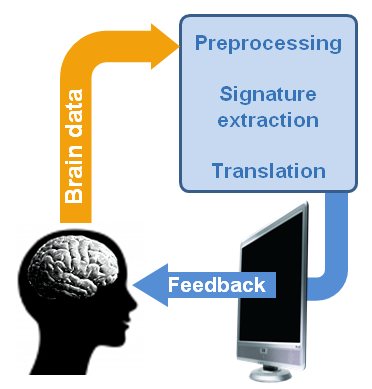
\includegraphics[scale=0.8]{Pictures/Chap1/bci_cycle_v2-2.png}
\caption{BCI 框架}
\label{Fig:bci_brief}
\end{figure}













\section{P300}


现在有很多测量脑信号的技术,如fMRI (functional magnetic resonance imaging,功能性磁共振成像),NIRS(near-infrared spectroscopy,近红外光谱学),EEG(Electroencephalograph,脑电图),MEG(Magnetoencephalography,脑磁图)等。针对不同的采集信号,其信号预处理方法也各不相同。但是BCI最基本的任务都是正确地识别“签名”并翻译成机器指令以完成用户的意愿。在P300拼写中,可以通过“oddball task”(如图\ref{Fig:P300_brief})产生P300信号。这个oddball task是一个关于字符注意的实验,展现一串字符(如SSTSSSSTSS),其中出现频率高的称为标准刺激(如该信号序列中的S),频率低的称为异常刺激(如该信号序列中的T)。当出现一个异常刺激时,300ms后就会在EEG信号中产生一个正向偏移。这里标准刺激和异常刺激的差异可以用来识别所给刺激的类别,然后基于刺激发送信号给计算机指令执行。
 
\begin{figure}[htb]
\centering
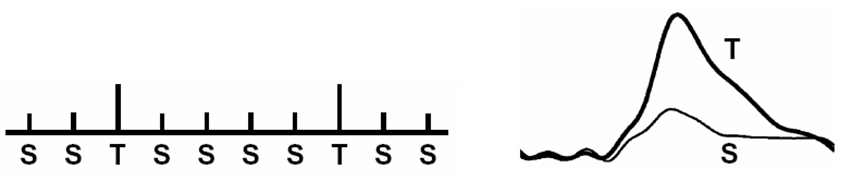
\includegraphics[scale=0.6]{Pictures/Chap1/p300_example.png}
\caption{P300刺激信号}
\label{Fig:P300_brief}
\end{figure}
Figure 2. 标准刺激(S)中的异常刺激(T)

在P300实验中,字母都展现在一个matrix中,其中同一时刻只有一行或一列亮起,具体哪一行或哪一列随机闪现。如下图所示,当一行一列相继闪烁的交点为指定字母时,测试者可以集中精神在头脑中进行简单计数或者确认,相应就会有P300产生。


\section{模版简介}

该模版以CTeX社区发布的ctexbook模版为基础,在数学系2006年模版上修改而来,删除了不兼容的旧代码,
增加了一些新版本扩展包支持的高级命令,部分功能实现方式与旧版有所不同。

该模版与研究生院网站发布的2008年模版排版效果基本相似,可直接使用。

该模版非学校官方模版,该模版可能引起的问题,{\bfseries{}模版作者不承担任何责任},特此声明。

\subsection{\LaTeX{}{}简介}

\LaTeX{}不是单指一个软件,而是指一类软件,这一类软件都是以一个基本软件\TeX\index{\TeX}为基础,
制作成宏包并经\TeX{}的原作者授权后发布。
打个比方,\TeX{}就是一些方形,三角形,圆形,半圆形的积木块,
\LaTeX{}就是另一些人用这些积木块搭成小房子,小桌子,
我们再把这些做好的小房子,小桌子摆摆成为我们的积木城市群,
就是这样。

为了国际化,\TeX{}不读“太可斯”,而按原作者Knuth, Donald Ervin的说法,
应读为“太chi”\cite{LaTeXshzh}。

Kunth是一个计算机与数学家,\TeX{}是其在1977年看到自己的成果出版时印刷质量甚不满意,
于是历时5年编写了\TeX{}排版系统,这成为西文排版业的一次重大革命。
\TeX{}系统于1982年正式定型,不再做大的改进,只修正发现的错误。
1989年,\TeX{}系统做了迄今为止最大的一次改进:支持多语言\cite{LaTeXshzh}。

\TeX{}的设计思想很简单:把一张纸看成一个坐标平面,将该坐标平面上哪一点要出现的内容标记出来,
就像这样:坐标(50,50),放置一个五号宋体的字,倾体,不加粗;从坐标(80,50)到坐标(80,200),
画一条粗为2的线,黑色……一个排好的版面就是这样被一个点一个点描述地画出来,Knuth设计的
\TeX{}指令,就是这些描述指令,然后由计算机解读,并做出最终的图,就是我们看到的排版效果。
\TeX 的精度很高,它的最小尺寸是一个叫做sp的小单位。可见光的波长近似等于100 sp,
几个sp 的误差眼睛是看不出来的\cite{texbook}。

从上面不难想到,如果只用\TeX 指令进行排版的话,会比较复杂,普通人难以胜任。
作为计算机专家的Knuth很清楚这一点,他给\TeX 设计了扩展接口。
利用这些接口,可以把\TeX 的一系列命令封装起来,做成各种各样的“宏”,这些宏,就被称为\LaTeX{}。
就像上面的比喻一样,用积木做小房子,小桌子的厂家有很多,于是就有了各种各样的\LaTeX{}版本:
MiKTeX,XeTeX,TeXLive,teTeX,fpTeX等。
使用\LaTeX{}模块,使得排版成为一件容易的事,尤其是使用已制作好的模版写文章,
不需要任务基础,知道几条语句就可以排出整齐统一的版面。
使用哪个版本的\LaTeX{}没有关系,都可以使用这个模版生成论文。这个模版制作使用的LaTeX版本是MiKTeX 2.9版。

\subsection{模版内容}

按照研究生院提供的2008版模版,毕业论文一共由封面、题名页、版权声明、勘误表、
致谢、序言、摘要、图表目录、术语表、目次、正文、参考文献、符录、索引、简历、文章列表,
一共十六部分组成\footnote{其实,还有脚注没有算上,脚注是隐含的,在这里\LaTeX{}将主动替你完成脚注的插入,而无需多作分心。就像这个脚注一样。}。

本模版将图表目录分成了图片目录与表格目录两个部分,因为这样一来清楚,二来\LaTeX{}原生支持图片与表格
分开作目录,作到一起反而费事。其它部分与研究生院模版相同。

在该模版中,任何一个部分都是可自由选择有无,如勘误表,大部分论文是没有这个部分的,
不需要某部分,只要将其生成语句注释掉即可,具体将在后面章节中讲解。
使用该模版,封面、题名页、版权声明、图片目录,表格目录、目次、参考文献、索引这八个部分不需要论文
作者直接参与,只需按要求在文中作出标记,\LaTeX{}就会替你自动生成这些部分,
而且完全不必考虑条目的编号顺序等问题。


